\chapter*{Remerciements}
Remerciements

\begin{abstract}
Extrait des conseils pour écrire un rapport de P3 et de Bachelor présents \href{https://gitlab-etu.ing.he-arc.ch/isc/documentation/projet-p3-et-bachelor/-/wikis/help-report}{ici} :
\begin{quote}    
  \begin{itemize}   
    \item Un résumé doit être compréhensible par tout le monde.
    \item Vous pouvez mettre une image, un schéma pour clarifier une explication.
    \item Vous devez décrire ce que fait votre application.
    \item Soyez positifs ! Commencez par dire tout ce qui fonctionne. Ne parlez qu’à la fin du résumé de choses négatives. Mais formulez de manière positive, par exemple plutôt que : « Ce logiciel n’est pas encore optimisé » écrire « Ce logiciel nécessiterait une optimisation, en particulier ... »  
  \end{itemize}
\end{quote}

\textbf{Mots-clefs :} les mots-clefs.
\end{abstract}

\renewcommand{\abstractname}{Abstract}
\begin{abstract}
Summary in EN.


\textbf{Keywords:} the keywords.
\end{abstract}

\todo[inline]{Juste pour vérifier l'équilibre du document. Ne garder qu'un niveau de 2 ou 3 à la fin}
\setcounter{tocdepth}{6}
\setcounter{secnumdepth}{6}
\tableofcontents

\clearpage
\pagenumbering{arabic} % Arabic (standard) page numbering

\chapter{Introduction}
Extrait des conseils pour écrire un rapport de P3 et de Bachelor présents \href{https://gitlab-etu.ing.he-arc.ch/isc/documentation/projet-p3-et-bachelor/-/wikis/help-report}{ici} :
\begin{quote}    
  \begin{itemize}   
    \item exposer le sujet (ou le thème, la matière prise en considération) en faisant valoir son importance et son originalité,
    \item articuler la problématique soulevée,
    annoncer le plan.
  \end{itemize}
\end{quote}

Pour inclure une image, il faut faire comme ceci :
\begin{figure}[h]
  \centering
  
\includegraphics[width=\textwidth]{./images/logos/he-arc-banner.jpg}
  \caption{Teaser figure.}
  \label{Fig_teaser}
\end{figure}

On peut ensuite facilement référencer la Figure \ref{Fig_teaser} ailleurs dans le texte.

Pour rajouter une nouvelle figure et la référencer (voir Figure \ref{Fig_exemple}).
\begin{figure}[h]
    \centering
    \includegraphics[width=0.5\textwidth]{./images/logos/he-arc-logo.png}
    \caption{Ceci est le nouveau logo de la HE-Arc.}
    \label{Fig_exemple}
\end{figure}

À noter que la numérotation se fait automatiquement.
Les liens entre les références sont aussi gérés de manière transparente.

\section{Comment formater le texte}
\textbf{Comment mettre un texte en gras.}
\underline{Comment souligner un texte.} 
\textit{Comment mettre un texte en italique.}
\underline{\textbf{\textit{On peut aussi mélanger les 3.}}}

Pour commencer un nouveau paragraphe, il suffit d'ajouter 1 ligne vide le fichier .tex.

Pour faire une liste :
\begin{itemize}
    \item élément 1
    \item élément 2
    \item élément 3
\end{itemize}

Pour faire une liste numérotée :
\begin{enumerate}
    \item élément 1
    \item élément 2
    \item élément 3
\end{enumerate}

\section{Lorem ipsum}
\lipsum[1-1] % PLACEHOLDER
\subsection{Dolor sit}
\lipsum[1-1] % PLACEHOLDER
\subsubsection{amet}
\lipsum[1-1] % PLACEHOLDER
\paragraph{consectetuer}
\lipsum[1-1] % PLACEHOLDER

\chapter{État de l'art}
Pour rajouter une référence sur un article, on fait comme ce qui suit :

"Besl et al. en 1992 \cite{besl_method_1992} présentent une technique de recalage appelée Iterative Closest Point (ICP dans la suite du document)."

Il est conseillé d'utiliser \href{https://www.zotero.org/}{Zotero} pour gérer sa bibliographie.

\section{Contributions}
Dans cette partie, il faut détailler les contributions apportées par rapport à l'état de l'art (en plus d'améliorer ses propres connaissances et d'acquérir de l'expérience).

\chapter{Analyse}
Il faut détailler le context du projet, les besoins, les spécifications, etc.

Quelle est la motivation derrière ce projet ? Qu'est-ce que ce projet apportera au final ?

On peut rajouter un diagramme WBS pour donner un aperçu haut-niveau :
\begin{figure}[h]
    \centering
    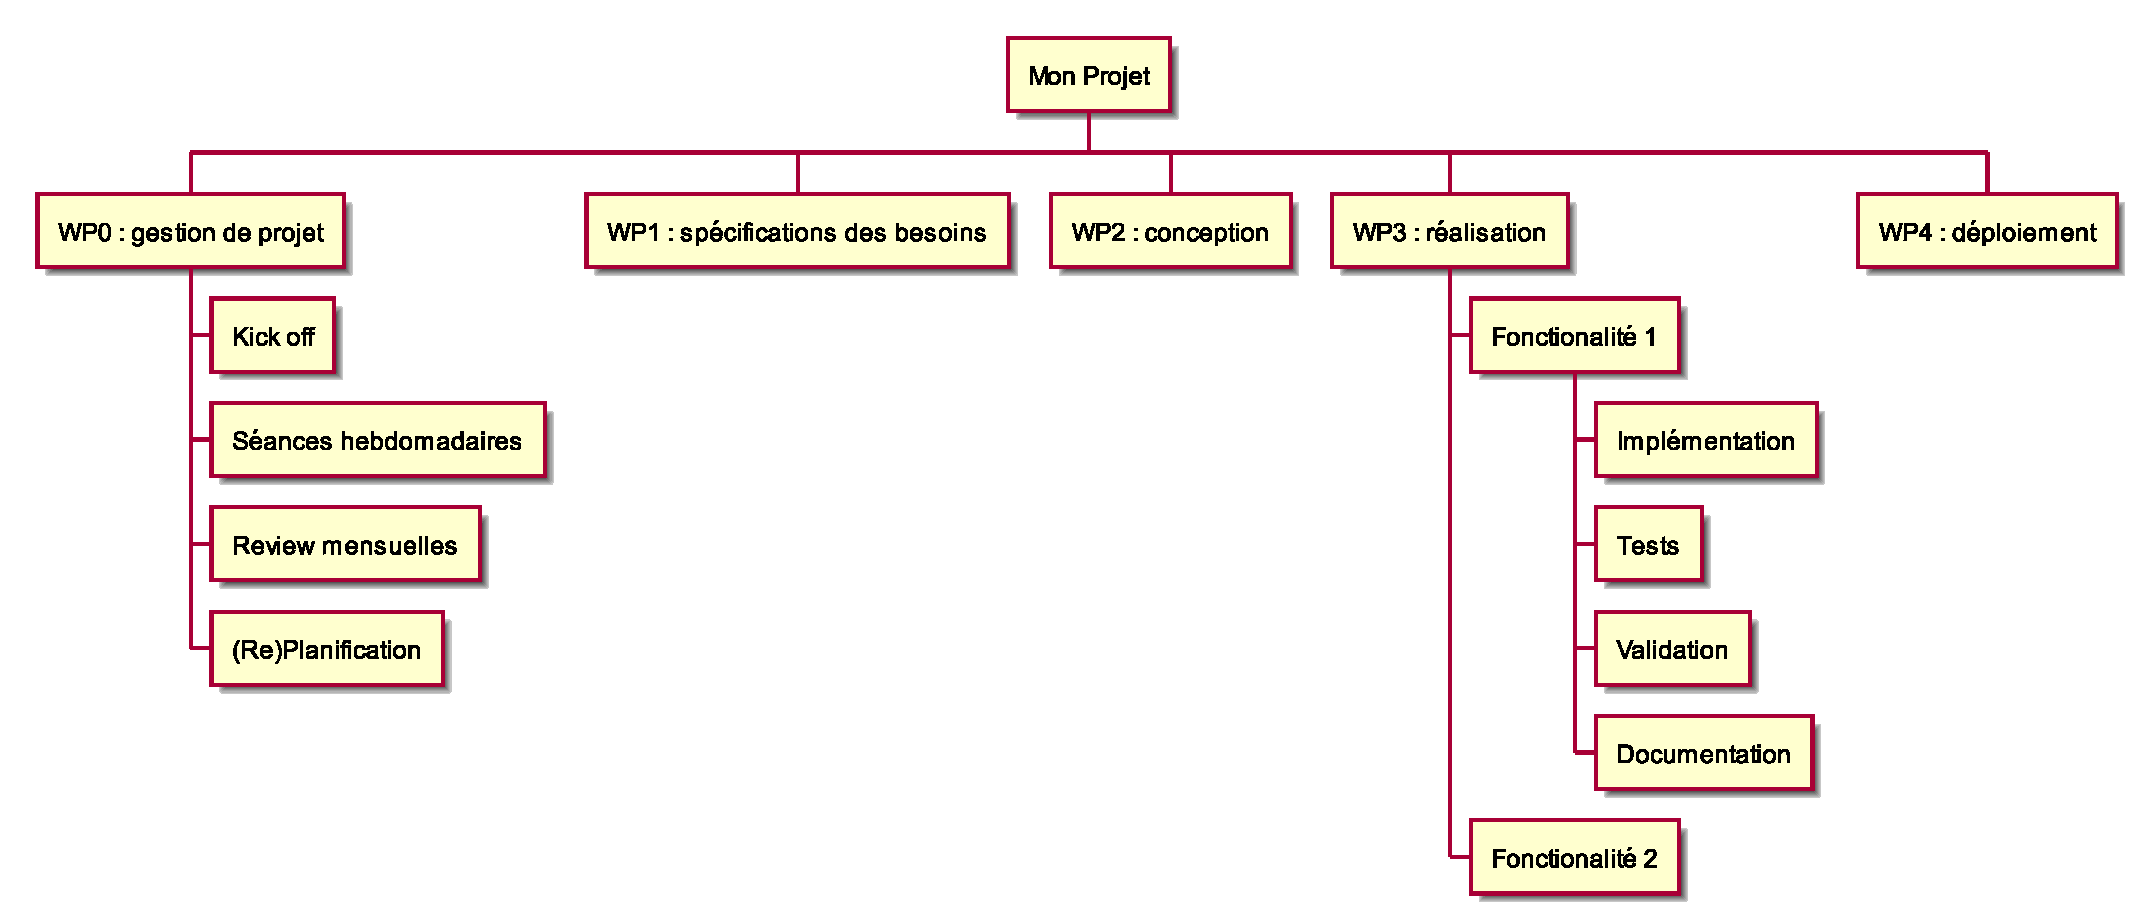
\includegraphics[width=\textwidth]{./images/WBS_Exemple.eps}
    \caption{Diagramme WBS qui va bien.}
\end{figure}

\section{Faisabilité}
Quels sont les contraintes de ce projet ? En quoi elles sont surmontables ? Un preuve de concept existe-t'elle déjà ?

\section{Risques}
Faire une analyse de risques et donner les solutions envisagées le cas échéant.
Pour chaque risque, il faut détailler les informations suivantes :
\begin{itemize}
  \item Son numéro;
  \item Son nom;
  \item Sa description;
  \item Sa probabilité : très improbable, improbable, probable, très probable;
  \item Son impact :  faible, modéré, grave, très grave;
  \item Niveau de criticité (Probabilité * Impact)
  \item Les mesures de prévention
  \item Les mesure de correction
\end{itemize}

Ensuite, on peut résumer ces informations dans un tableau comme ce qui suit :

\begin{tabular}{ | l | l | l | l | }
  N° & Nom & Probabilité & Impact \\
  \rowcolor{red!60}
  01 & Risque critique & probable & grave \\
  \rowcolor{red!20}
  02 & Risque acceptable & probable & faible \\
  03 & Risque insignifiant & peu probable & faible
\end{tabular}

\section{Planification}
Il faut rajouter un diagramme de Gantt ici.

\section{Technologies utilisées}
Expliquer les choix concernant les technologies.
Si possible, montrer les avantages et les inconvénients de chaque technologie pour justifier ses choix.
Si un prototype est créé pour tester des points chauds, c'est intéressant de le mentionner ici.

\chapter{Conception}
Dans cette partie, montrer les différents diagrammes UML utilisés.
Il est conseillé d'utiliser \href{https://plantuml.com/}{PlantUML} car il permet de générer des diagrammes UML décrits par du "code".

Une partie sur la gestion de projet (Gitlab, Kanban, Issues, Milestones, etc.) peut aussi être intéressante.

Pour les algorithmes, vous pouvez faire comme ce qui suit :

\begin{algorithm}[H]
\SetAlgoLined
\KwResult{Super résultat}
x, y, z $\leftarrow$ 0\;
\While{condition}
{
  instructions\;  
  \eIf{condition}
  {
    instructions1\;
    instructions2\;
  }
  {
   instructions3\;
  }
}
\For{condition}
{
  instructions\;  
  \eIf{condition}
  {
    instructions1\;
    instructions2\;
  }
  {
   instructions3\;
  }
}
\caption{Mon algorithme}
\end{algorithm}

\chapter{Implémentation}
Pour afficher des instructions en ligne de command, vous pouvez faire comme ceci :
\begin{commandline}
  \begin{verbatim}
	$ git pull --rebase
	\end{verbatim}
\end{commandline}

Pour attirer l'attention de lecteur sur un point intéressant :
\begin{info}[Bon à savoir :]
 	Ceci est une information intéressante à mettre en avant dans le rapport.
\end{info}

Pour avertir de lecteur :
\begin{warn}[Erreur à éviter :]
 	Ceci est une erreur fréquente qu'il faut absolument éviter.
\end{warn}

Si vous avez besoin de lister un (petit) bout de code, il faut faire comme ce qui suit :
\begin{lstlisting}
// This is great!
IEnumerator DoCheck() 
{
  for(;;)
  {
    ProximityCheck();
    Debug.Log("Yielding execution here");
    yield return new WaitForSeconds(.1f);
    Debug.Log("Execution resumed");
  }
}
\end{lstlisting}

\chapter{Résultats}

\chapter{Limitations et perspectives}

\chapter{Conclusion}